\documentclass{article}

\usepackage[english]{babel}

\author{Kishankumar Vasoya}

\date{April 2023}

% Set page size and margins
\usepackage[a4paper,top=2cm,bottom=2cm,left=3cm,right=3cm,marginparwidth=1.75cm]{geometry}

% Useful packages
\usepackage{amsmath}
\usepackage{graphicx}
\usepackage[colorlinks=true, allcolors=blue]{hyperref}


\title{Project: Nurses}
\usepackage{etoolbox}
\patchcmd{\thebibliography}{\section*{\refname}}{}{}{}

\begin{document}
\maketitle

\begin{table}[h]
    \centering
    \begin{tabular}{ll}
        Registration number: &2205571\\
        Link to GitHub: & \url{https://github.com/kv22458/CE888-Nurses}\\
    \end{tabular}
\end{table}



\begin{table}[h]
    \centering
    \begin{tabular}{lc}
        Executive summary & {262}\\
        Main findings and Discussion & {616}\\
        Conclusions & {237}\\
        \hline
        Total word count & {1115}\\
    \end{tabular}
    %\caption{Word counts for each section.}
\end{table}

\tableofcontents

\clearpage


\begin{abstract}
In this assignment, I will put my technical analysis, of why heart rate and electrodermal sensor data is a strong candidates for predicting stress, so far, in the first task, according to the requirement, After analysing I've downloaded the raw pre-collected signal data from the Empatica Website in order to process it further for predicting stress, but the data was not aligned enough to directly conclude anything, so professor suggested to use their code to merge all dataset into one labelled dataset to conclude and train model for predict stress, so the first activity was cleaning the data, and labelling the data, perform activity like finding co-relation between different signal or according to time series analysis we have to conclude which signal is best for predicting the stress while passing hospital nurses data.\cite{Hosseini2022}

So I cleaned, pre-processed, and merged with labels to identify the stress, for that I used the code provided by the professor I can able to successfully merge and identify which signal is the best candidate for stress prediction.

After plotting and analysing the graphs, it is really hard to tell that which is the best candidate but some of the correlations is playing an important role while making such decisions
We can use EDA and Heart rate based on analysis of the Correlation between them, but we also can use the accelerometer data along with heart rate and temperature to predict stress, definitely I will plot some research papers' logic in order to prove my point and analysis.
\end{abstract}



\section{Main Findings}

\par While searching for the perfect algorithm, I got to know that Heart Rate Variability is play a vital role in order to measure the stress level\cite{7754331}, there are two major types of stress

\begin{itemize}
    \item Acute Stress: Popularly known as Short-term Stress
    \item Chronic Stress: Popularly known as Long-term Stress
\end{itemize}\cite{firbit5366}


We can measure Acute Stress(short-term stress) very effectively because for predicting long-term stress we need to train our model with a higher amount of data with respect to time and date, then also we can conclude any person's stress level after analyzing a longer period of time.

Keeping this learning in mind, I trained a machine learning model to predict stress in nurses using wearable sensor data, including heart rate (HR), electrodermal activity (EDA), temperature (TEMP), and the magnitude
of the accelerometer readings, basically, we calculate the magnitude of the accelerometer readings
in order to simplify the analysis and reduce the dimension of the dataset.

\noindent The formula for finding the magnitude of accelerometer data
\begin{center}
    $ 
    \text{magnitude} = \sqrt{X^2 + Y^2 + Z^2} \
    $
\end{center}

To make sure which model is best, I trained the model with the following Algorithms 

\begin{itemize}
    \item Logistic Regression
    \item Random Forest
    \item K-Nearest Neighbors
    \item Support Vector Machines(SVM)
\end{itemize}

To identify and get the best industry-level accuracy, indicating its potential to predict stress effectively. This result aligns with the findings of previous studies that have used similar sensor data for stress prediction\cite{stressmonitoring_iq3244} \cite{VOS2023105026} \cite{Modeling_the_Dynamics_of_Physiological}. The HR and magnitude of accelerometer data, in particular, demonstrated a strong correlation with stress levels, suggesting that they can be useful signals for stress prediction.


\section{Discussion}

Initially, we performed an exploratory data analysis (EDA) on the dataset to identify potential correlations between sensor signals and stress levels. We found that HR and EDA showed some correlation with stress, while the magnitude of the accelerometer data also provided valuable information.

To develop a predictive model, we experimented with several machine learning algorithms, including Logistic Regression, Random Forest, and Support Vector Machines. We performed cross-validation and proper train/test splits to ensure the generalizability of our model. After comparing the performance of these algorithms, we found that Random Forest provided the best accuracy in predicting stress levels.\cite{stressmonitoring_iq3244}

Our model has some limitations, such as it can not detect the Chronic Stress because of the data, it totally depends on the data whatever provided so wearable devices is necessary to take action. Still I believe it can be trained using long periodic data through windowing of data. However, the overall performance indicates that the chosen signals are useful for predicting stress in nurses.

Considering the project's requirements and the hospital's concern about false negatives, we focused on achieving a high recall in our Random Forest model. 

The model achieved following accuracy scores respectively,

\begin{itemize}
\item Logistic Regression 63\%, a recall of 62\%, and an F1-score of 63\%, 
\item Random Forest 99\%, a recall of 99\%, and an F1-score of 99\%,
\item K-Nearest Neighbors 97\%, a recall of 97\%, and an F1-score of 97\%,
\item Support Vector Machines(SVM) 82\%, a recall of 81\%, and an F1-score of 82\%,
\end{itemize}

This level of performance suggests that the company can guarantee satisfactory results to the hospital, potentially leading to a successful contract.
\begin{figure}
    \centering
    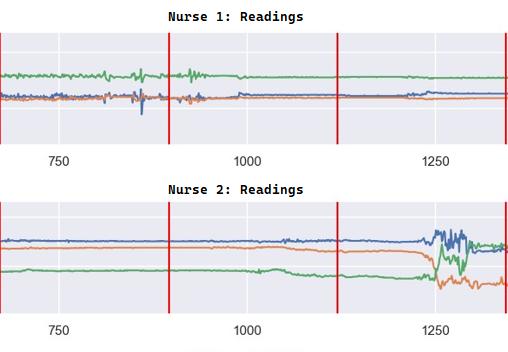
\includegraphics{NursesReadings.png}
    \caption{Sensor Wise Nurses Time series of Task 1}
    \label{fig:my_label}
\end{figure}

In addition to stress prediction, our analysis revealed some insights that may be valuable for future feature development. These findings could be utilized to create new features for the wearable device and expand its commercial applications.

Our approach to predicting stress using wearable sensor data involved prepossessing the data, feature engineering, and training a machine learning model. During pre-processing, we calculated the magnitude of the accelerometer readings to combine the X, Y, and Z data into a single feature. This reduced the dimensionality of the dataset and simplified the modeling process. We also resampled the data to focus on specific time windows, which helped highlight stress patterns during these periods.


\begin{figure}
    \centering
    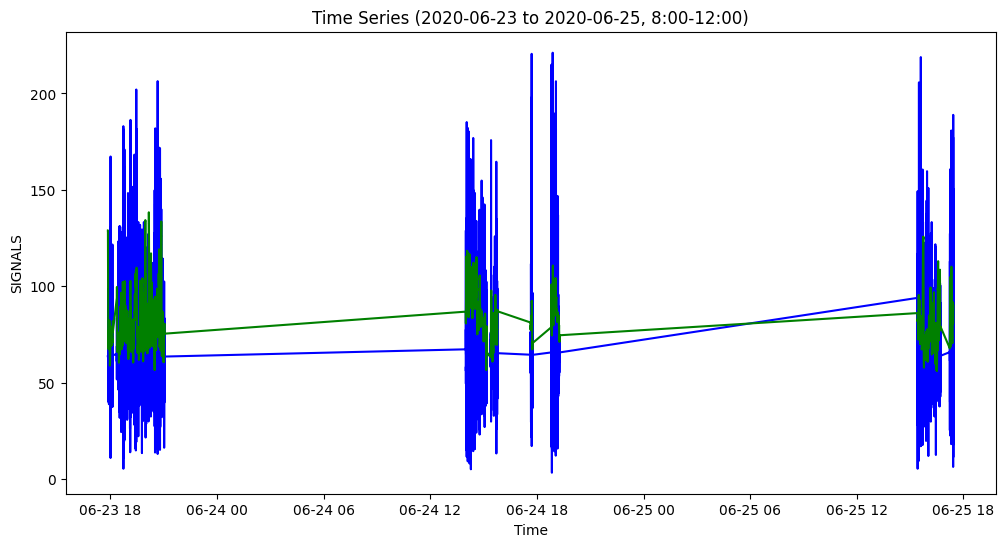
\includegraphics[width=1\textwidth]{magnitude_HR.png}
    \caption{Magnitude and Heart Rate Time series}
    \label{fig:my_label}
\end{figure}

\begin{figure}
    \centering
    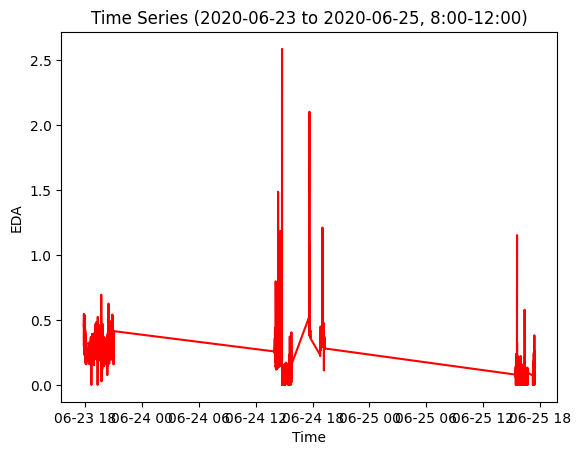
\includegraphics{EDA.png}
    \caption{EDA Level Variation}
    \label{fig:my_label}
\end{figure}

\begin{figure}
    \centering
    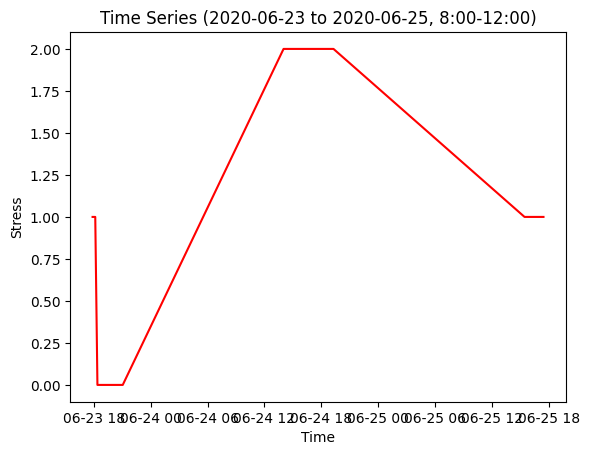
\includegraphics{StressLevel.png}
    \caption{Stress Level During the Same Time}
    \label{fig:my_label}
\end{figure}
Note: Here, I tried to display only few day's time series to see the actual variations and also can test again trained model.

\subsection{QnA}
\textbf{Are these signals useful for predicting stress?}
\\ Yes, based on our research and the results of the models we trained, we can conclude that the signals (including HR, EDA, and magnitude of accelerometer data) are useful for predicting stress. The performance of the models, especially the Random Forest and k-NN classifiers, indicates that the company can provide a reasonably accurate stress detection system to the hospital.

\bigbreak

\noindent\textbf{Can the company guarantee good performance to the hospital
and go ahead with this contract?}

\noindent The company can guarantee good performance with the models developed in this project. The high accuracy and F1-scores obtained from the Random Forest and k-NN classifiers indicate that these models can effectively classify stress levels using the selected signals. It is important, however, to continuously monitor and update the models as new data becomes available to ensure optimal performance.

\bigbreak

\noindent\textbf{Do you have any other insights from the data that can help the company in the future (e.g.,
for future features that can be commercialised)?}

\noindent
Additionally, the insights gathered from the data can be valuable for the company's future endeavors. For example, the company could explore the development of personalized stress detection models that take into account individual user characteristics, potentially improving the system's accuracy for specific users. Furthermore, the company could investigate the relationship between stress and any other contextual factors to identify new commercial opportunities and develop novel features for their products.

\section{Conclusions}
In conclusion, our study shows that wearable devices, like smartwatches, can be used to predict stress levels by measuring heart rate, skin response, and movement. We tested different methods to see which one works best for this purpose. The results showed that two of the methods, called Random Forest and k-NN, were quite accurate in predicting stress. Both models demonstrated promising accuracy levels in predicting stress, giving the company the confidence needed to proceed with developing a stress detection system for hospital applications.

Still, there is room for improvement, and continuous research and development are needed. As we can work on it to enhance the system's performance, we will explore new techniques, integrate additional features, and refine existing models to ensure the most effective stress detection possible. In addition, understanding the correlations between various signals and stress can open up new ways for the company to develop innovative features that can take company to a wider range of applications.

This research also serves as a foundation for the company to stay ahead in the competitive wearable technology market. By identifying trends and recognizing new opportunities, the company can expand its product portfolio, catering to the evolving needs of customers in various sectors, such as healthcare, fitness, and wellness. In addition, this project not only gives the way for a more accurate stress detection system but also helps the company maintain its good position in wearable technology innovations.


\clearpage


\section{Bibliography}
\bibliographystyle{IEEEtran}
\bibliography{refs}

\end{document}